\documentclass[border=5pt]{standalone}
\usepackage[scaled]{helvet}
\renewcommand\familydefault{\sfdefault} 
\usepackage[T1]{fontenc}
\usepackage{tikz}
\usepackage{xcolor}
\usepackage{amssymb}
\usepackage{enumitem}
\usetikzlibrary{shapes.geometric, shapes.multipart, shapes.arrows, arrows.meta, positioning, shadows, calc}

% Define colors matching the image and historical transitions
\definecolor{box1head}{RGB}{140, 140, 140} % Gray
\definecolor{box1body}{RGB}{245, 245, 245}
\definecolor{box2head}{RGB}{205, 140, 60}  % Mute Orange
\definecolor{box2body}{RGB}{252, 245, 235}
\definecolor{box3head}{RGB}{169, 214, 229} % Light Blue
\definecolor{box3body}{RGB}{235, 248, 252}
\definecolor{box4head}{RGB}{69, 145, 143} % Teal
\definecolor{box4body}{RGB}{236, 247, 245}
\definecolor{box5head}{RGB}{25, 48, 72}   % Navy Blue

\begin{document}

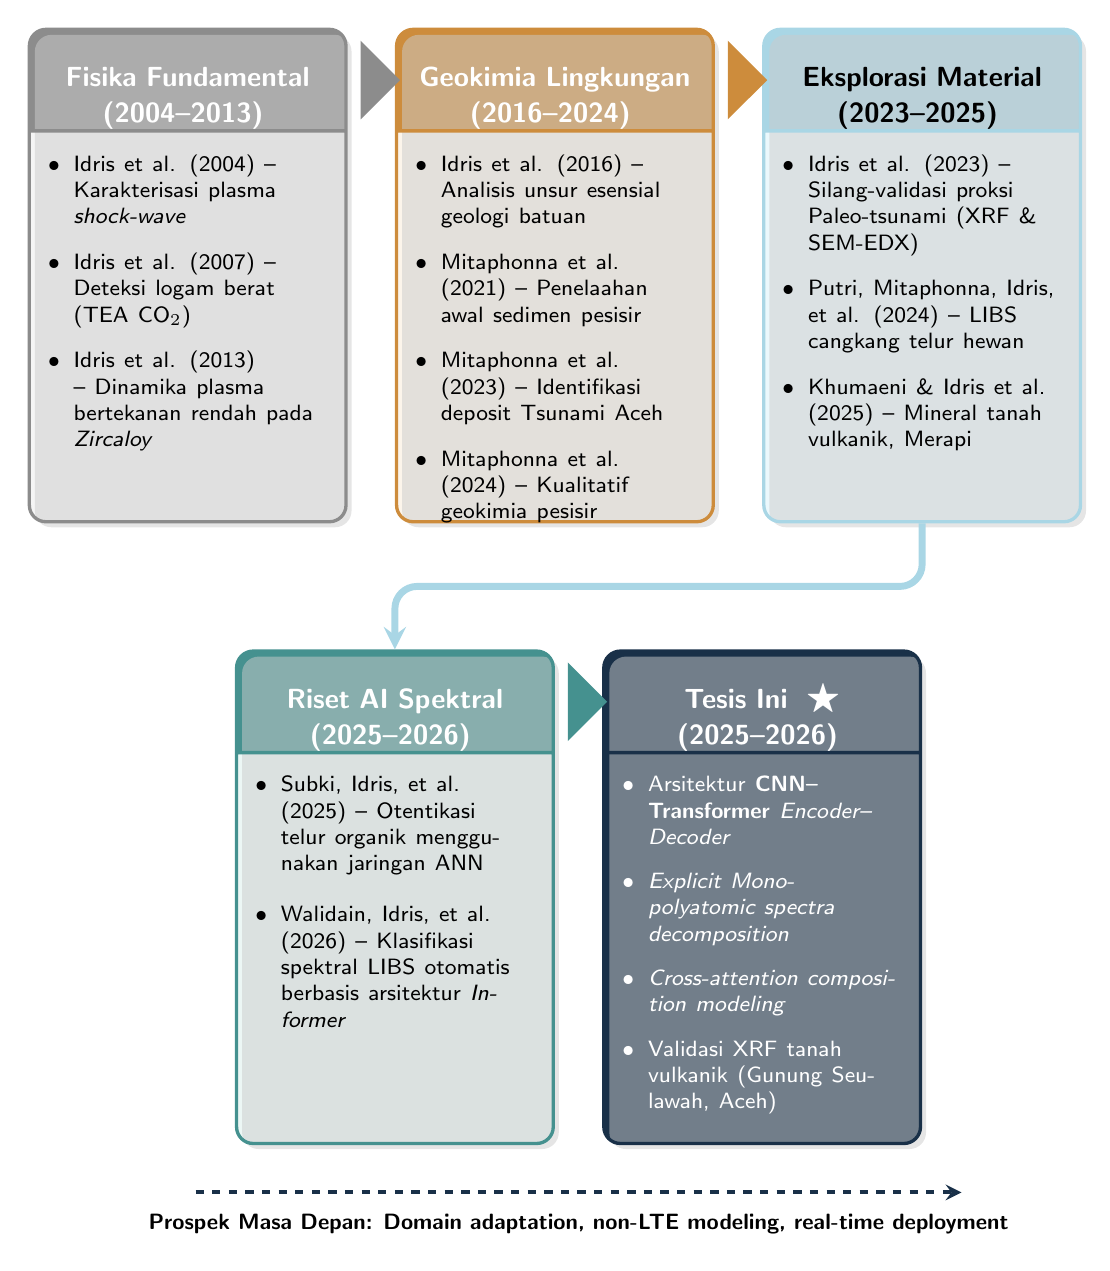
\begin{tikzpicture}[
    > = stealth,
    font=\sffamily,
    % Multipart box style definition
    splitbox/.style 2 args={
        rectangle split,
        rectangle split parts=2,
        rounded corners=6pt,
        draw=#1,
        line width=1.2pt,
        rectangle split part fill={#1, #2},
        text width=3.6cm, % slightly wider
        inner xsep=6pt,
        inner ysep=6pt,
        drop shadow={color=gray!40, shadow xshift=2pt, shadow yshift=-2pt}
    },
    % Arrow style
    myarrow/.style={
        single arrow, minimum height=0.5cm, minimum width=1.0cm, 
        single arrow head extend=1.5mm, draw=none
    }
]

% ================= ROW 1: 3 BOXES =================
% GROUP 1
\node[splitbox={box1head}{box1body}] (box1) {
    \nodepart{one}
    \begin{center}
        \vspace{-6pt}
        \textbf{\color{white}\normalsize Fisika Fundamental\\[1pt](2004--2013)}
        \vspace{-6pt}
    \end{center}
    
    \nodepart{two}
    \begin{minipage}[t][4.5cm]{3.5cm}
    \vspace{2pt}
    \begin{itemize}[leftmargin=10pt, label={\color{black}$\bullet$}, itemsep=3pt]\footnotesize\color{black}
        \item Idris et al. (2004) -- Karakterisasi plasma \textit{shock-wave}
        \item Idris et al. (2007) -- Deteksi logam berat (TEA CO$_2$)
        \item Idris et al. (2013) -- Dinamika plasma bertekanan rendah pada \textit{Zircaloy}
    \end{itemize}
    \end{minipage}
};

% GROUP 2
\node[splitbox={box2head}{box2body}, right=0.6cm of box1] (box2) {
    \nodepart{one}
    \begin{center}
        \vspace{-6pt}
        \textbf{\color{white}\normalsize Geokimia Lingkungan\\[1pt](2016--2024)}
        \vspace{-6pt}
    \end{center}
    
    \nodepart{two}
    \begin{minipage}[t][4.5cm]{3.5cm}
    \vspace{2pt}
    \begin{itemize}[leftmargin=10pt, label={\color{black}$\bullet$}, itemsep=3pt]\footnotesize\color{black}
        \item Idris et al. (2016) -- Analisis unsur esensial geologi batuan
        \item Mitaphonna et al. (2021) -- Penelaahan awal sedimen pesisir
        \item Mitaphonna et al. (2023) -- Identifikasi deposit Tsunami Aceh
        \item Mitaphonna et al. (2024) -- Kualitatif geokimia pesisir
    \end{itemize}
    \end{minipage}
};

% GROUP 3
\node[splitbox={box3head}{box3body}, right=0.6cm of box2] (box3) {
    \nodepart{one}
    \begin{center}
        \vspace{-6pt}
        \textbf{\color{black}\normalsize Eksplorasi Material\\[1pt](2023--2025)}
        \vspace{-6pt}
    \end{center}
    
    \nodepart{two}
    \begin{minipage}[t][4.5cm]{3.5cm}
    \vspace{2pt}
    \begin{itemize}[leftmargin=10pt, label={\color{black}$\bullet$}, itemsep=3pt]\footnotesize\color{black}
        \item Idris et al. (2023) -- Silang-validasi proksi Paleo-tsunami (XRF \& SEM-EDX)
        \item Putri, Mitaphonna, Idris, et al. (2024) -- LIBS cangkang telur hewan
        \item Khumaeni \& Idris et al. (2025) -- Mineral tanah vulkanik, Merapi
    \end{itemize}
    \end{minipage}
};

% ================= ROW 2: 2 BOXES =================
% Position anchors
\path (box1.south east) -- (box2.south west) coordinate (mid12);
\path (box2.south east) -- (box3.south west) coordinate (mid23);

% GROUP 4
\node[splitbox={box4head}{box4body}, below=1.6cm of mid12, anchor=north] (box4) {
    \nodepart{one}
    \begin{center}
        \vspace{-6pt}
        \textbf{\color{white}\normalsize Riset AI Spektral\\[1pt](2025--2026)}
        \vspace{-6pt}
    \end{center}
    
    \nodepart{two}
    \begin{minipage}[t][4.5cm]{3.5cm}
    \vspace{2pt}
    \begin{itemize}[leftmargin=10pt, label={\color{black}$\bullet$}, itemsep=5pt]\footnotesize\color{black}
        \item Subki, Idris, et al. (2025) -- Otentikasi telur organik menggunakan jaringan ANN
        \item Walidain, Idris, et al. (2026) -- Klasifikasi spektral LIBS otomatis berbasis arsitektur \textit{Informer}
    \end{itemize}
    \end{minipage}
};

% GROUP 5
\node[splitbox={box5head}{box5head}, below=1.6cm of mid23, anchor=north] (box5) {
    \nodepart{one}
    \begin{center}
        \vspace{-6pt}
        \textbf{\color{white}\normalsize Tesis Ini\ \ \scalebox{1.3}{$\bigstar$}\\[1pt](2025--2026)}
        \vspace{-6pt}
    \end{center}
    
    \nodepart{two}
    \begin{minipage}[t][4.5cm]{3.5cm}
    \vspace{2pt}
    \begin{itemize}[leftmargin=10pt, label={\color{white}$\bullet$}, itemsep=2.5pt]\footnotesize\color{white}
        \item Arsitektur \textbf{CNN--Transformer} \textit{Encoder--Decoder}
        \item \textit{Explicit Mono-polyatomic spectra decomposition}
        \item \textit{Cross-attention composition modeling}
        \item Validasi XRF tanah vulkanik (Gunung Seulawah, Aceh)
    \end{itemize}
    \end{minipage}
}; 

% ================= HORIZONTAL ARROWS =================
\path (box1.east |- box1.one east) -- (box2.west |- box2.one west) 
    node[midway, myarrow, fill=box1head] {};
\path (box2.east |- box2.one east) -- (box3.west |- box3.one west) 
    node[midway, myarrow, fill=box2head] {};
\path (box4.east |- box4.one east) -- (box5.west |- box5.one west) 
    node[midway, myarrow, fill=box4head] {};

% ================= WRAP AROUND U-TURN ARROW (Row 1 -> Row 2) =================
\draw [line width=2.5pt, box3head, -stealth, rounded corners=8pt] 
    (box3.south) -- +(0,-0.8cm) -| (box4.north);

% ================= BOTTOM TIMELINE =================
% Position line perfectly aligned with bottom boxes
\draw[box5head, dashed, line width=1.5pt, ->] 
    ($(box4.south west) + (-0.5cm, -0.6)$) -- ($(box5.south east) + (0.5cm, -0.6)$);

% Position text cleanly below
\node[align=center, font=\footnotesize\bfseries, text=black] 
    at ($($(box4.south west) + (-0.5cm, -1.0)$)!0.5!($(box5.south east) + (0.5cm, -1.0)$)$) 
    {Prospek Masa Depan: Domain adaptation, non-LTE modeling, real-time deployment};

\end{tikzpicture}
\end{document}
